\section{Preliminares}

\subsection{Árboles de Búsqueda Binaria (ABBs)}

Un árbol de búsqueda binaria o ABB es una estructura que permite guardar los elementos
de un conjunto finito totalmente ordenado \(X\), es decir,
que todo par de elementos \(x, y \in X\), es \textit{comparable}, es decir, exactamente uno de los siguientes es verdadero: 

\[ x < y \qquad x = y \qquad  x > y \]

En cada nodo $x$ del árbol se guarda un valor del conjunto, y posee además dos hijos (potencialmente nulos),
llamados izquierdo y derecho, con la propiedad que el hijo izquierdo es un ABB del conjunto
$X_< = \{ y \in X : y < x \}$; y el hijo derecho es un ABB del conjunto $X_> = \{y \in X : y > x\}$.
Notar que no pueden haber dos nodos con el mismo valor, por cómo se definen estos conjuntos.

En nuestro caso, $X$ va a ser un subconjunto de \( \mathbb{Z} \), el conjunto de números enteros.
Podemos pensar que cada nodo del ABB representa un intervalo,
de manera que cada nivel del árbol (los nodos a una cierta profundidad) es una partición de \(\mathbb{Z}\) menos los elementos que hay en niveles superiores.

\begin{center}
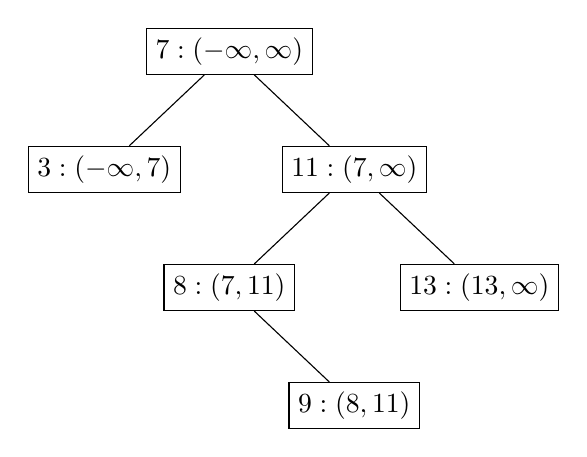
\begin{tikzpicture}[
sibling distance=1.25in,
every node/.style={draw}
]
\node {\(7: (-\infty, \infty)\)}
    child { node {\(3: (-\infty, 7)\)} }
    child { node {\(11: (7, \infty)\)} 
        child { node {\(8: (7, 11)\)}
            child [missing]
            child { node {\(9: (8, 11)\)}}
        }
        child { node {\(13: (13, \infty)\)}}
    };
\end{tikzpicture}
\captionof{figure}{Particionar niveles en intervalos}
\end{center}

\vbox{
El árbol soporta tres operaciones sobre el conjunto:

\begin{enumerate}
    \item Buscar(\(x\)), que dice si \(x\) pertenece o no al conjunto
    \item Insertar(\(x\)), que inserta \(x\) en el conjunto
    \item Borrar(\(x\)), que elimina \(x\) del conjunto
\end{enumerate}
}

Estas tres operaciones cuestan $\mathcal{O}(h)$,
donde $h$ es la máxima profundidad de un nodo (también llamada la altura del árbol).
Como cada nivel $k$ tiene a lo sumo $2^k$ nodos, $h \geq \lceil \lg |X| \rceil$.
En el peor de los casos, puede ocurrir que $h = n$.

Por esta razón, existen los Árboles de Búsqueda Binaria Auto-Balanceables,
que garantizan que \(h = \mathcal{O}(\lg n)\), como el caso de árboles AVL o Red-Black.
En el caso del Treap, se realiza esta misma cota con muy alta probabilidad.

\subsection{Heaps}

Un \textit{Heap} (binario), también conocido como "Montículo", es otra clase de árbol binario,
que guarda un valor en cada nodo, y mantiene la propiedad que todo nodo tiene
el valor máximo en su subárbol.

\begin{center}
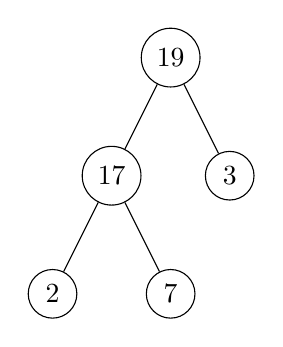
\begin{tikzpicture}[
every node/.style={circle,draw}
]
\node {\(19\)}
    child {node {\(17\)}
        child {node {\(2\)}}
        child {node {\(7\)}}
    }
    child {node {\(3\)}};
\end{tikzpicture}
\captionof{figure}{Ejemplo de un Heap}
\end{center}

Se pueden insertar y eliminar nodos en $\mathcal{O}(\lg n)$, y acceder al máximo elemento en tiempo constante.
Sin embargo, en nuestro caso, no nos va a interesar usarlo como estructura de datos,
sino que vamos a usar la forma del árbol determinada por los valores.